\chapter{Chapter 3 Supplementary Content}\label{app:ch3suppcontent}
\myappendices{Appendix \ref{app:ch3suppcontent}: Chapter 3 Supplementary Content}
\newpage

\section{Prediction Accuracy across all landmarks}\label{app:Chap}

\begin{table}[H]
\centering
\small
\caption{Per-landmark prediction accuracy of AutoAFIDs. Values represent the Euclidean Distance (ED) between predicted and ground truth landmark coordinates across 21 test subjects.}
\label{tab:autoafids_accuracy}
\begin{tabular}{lcccc}
\toprule
\textbf{Landmark} & \textbf{Median (mm)} & \textbf{IQR (mm)} & \textbf{Min (mm)} & \textbf{Max (mm)} \\
\midrule
AFID 1  & 0.42 & 0.29--0.69 & 0.04 & 1.53 \\
AFID 2  & 0.83 & 0.73--1.14 & 0.37 & 1.32 \\
AFID 3  & 0.90 & 0.65--1.09 & 0.36 & 2.06 \\
AFID 4  & 0.73 & 0.58--0.95 & 0.15 & 2.08 \\
AFID 5  & 0.80 & 0.60--1.12 & 0.29 & 2.46 \\
AFID 6  & 1.57 & 1.04--1.78 & 0.42 & 2.37 \\
AFID 7  & 1.26 & 0.86--1.55 & 0.24 & 2.39 \\
AFID 8  & 2.11 & 1.60--3.73 & 0.52 & 5.30 \\
AFID 9  & 1.41 & 1.07--2.43 & 0.51 & 3.99 \\
AFID 10 & 1.30 & 0.87--2.02 & 0.52 & 3.73 \\
AFID 11 & 1.23 & 0.80--1.74 & 0.29 & 3.62 \\
AFID 12 & 1.37 & 0.90--2.11 & 0.51 & 3.77 \\
AFID 13 & 1.23 & 0.88--1.86 & 0.44 & 3.63 \\
AFID 14 & 1.03 & 0.79--1.41 & 0.38 & 2.64 \\
AFID 15 & 1.04 & 0.85--1.65 & 0.36 & 2.26 \\
AFID 16 & 1.09 & 0.87--1.47 & 0.57 & 2.25 \\
AFID 17 & 1.00 & 0.85--1.22 & 0.32 & 1.94 \\
AFID 18 & 1.20 & 0.96--1.51 & 0.49 & 2.67 \\
AFID 19 & 1.26 & 1.05--1.85 & 0.47 & 2.93 \\
AFID 20 & 1.36 & 0.97--1.93 & 0.61 & 2.81 \\
AFID 21 & 1.38 & 1.00--1.99 & 0.41 & 3.36 \\
AFID 22 & 1.27 & 0.79--1.69 & 0.34 & 2.64 \\
AFID 23 & 1.16 & 0.53--1.69 & 0.10 & 3.31 \\
AFID 24 & 2.28 & 1.53--2.67 & 0.35 & 4.12 \\
AFID 25 & 2.28 & 1.66--3.27 & 0.64 & 6.21 \\
AFID 26 & 2.08 & 1.45--2.94 & 1.15 & 6.66 \\
AFID 27 & 1.47 & 0.80--2.10 & 0.21 & 4.31 \\
AFID 28 & 1.56 & 1.21--1.87 & 0.55 & 3.36 \\
AFID 29 & 1.79 & 1.38--2.46 & 0.70 & 3.61 \\
AFID 30 & 2.21 & 1.18--2.78 & 0.35 & 4.70 \\
AFID 31 & 1.19 & 0.91--1.63 & 0.34 & 2.98 \\
AFID 32 & 1.00 & 0.79--1.69 & 0.12 & 2.64 \\
\midrule
\textbf{All AFIDs} & \textbf{1.21} & \textbf{0.76--1.95} & \textbf{0.04} & \textbf{6.66} \\
\bottomrule
\end{tabular}
\end{table}

\newpage
\section{registration quality control file}
AutoAFIDs provides an optional registration quality control (QC) module that generates subject-level HTML reports to assess the fidelity of spatial normalization. For each subject, the tool computes standard summary statistics of landmark error, including minimum, maximum, mean, median, standard deviation, and interquartile range across all 32 anatomical fiducials. Visualizations include (i) slice-based qualitative review panels with crosshair overlays in sagittal, coronal, and axial views, (ii) a color-coded heatmap of per-landmark errors across x, y, z axes and Euclidean distance, and (iii) a 3D scatterplot showing the displacement between predicted subject landmarks and reference coordinates in stereotactic space. The report enables both quantitative inspection and visual verification of anatomical alignment and can be integrated into larger processing workflows for automated QC flagging.

The registration QC module in AutoAFIDs can be invoked as part of the BIDS-App command-line interface. To enable QC report generation, users must provide a directory containing their Lead-DBS derivative files. A typical invocation is shown below:

\begin{verbatim}
autoafids <BIDS_DIR> <DERIVATIVES_DIR> participant
--LEAD-DBS-DIR <PATH_TO_LEAD-DBS_Directory>
\end{verbatim}

This command runs the QC module on all subjects found in the BIDS directory, compares registered AFIDs to reference space, and saves the resulting HTML reports to the specified output directory. Each report includes per-subject error statistics, slice-wise visual inspection panels, a heatmap of landmark errors, and a 3D displacement plot. This functionality is integrated into the default workflow and designed for seamless use in automated pipelines.
\begin{figure}
    \centering
    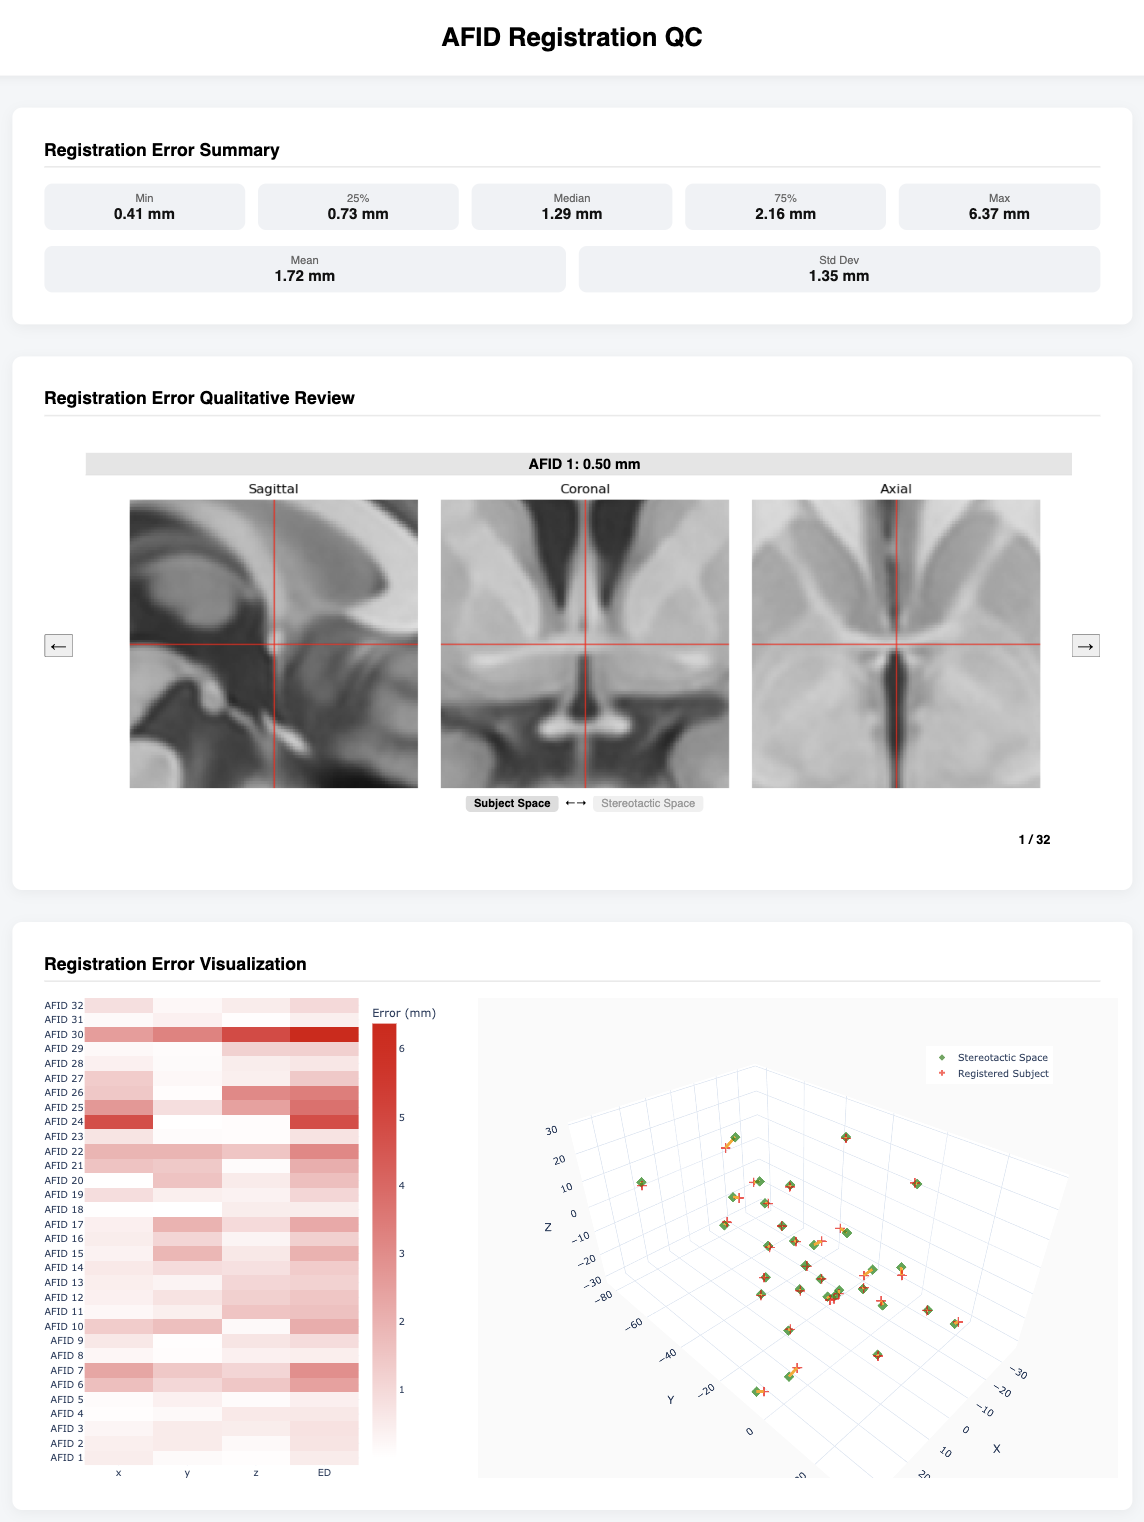
\includegraphics[width=0.95\linewidth]{figs/figuresupregqc.png}
    \caption{Example AutoAFIDs registration QC report for one subject.}
    \label{fig:figuresupregqc}
\end{figure}